% Dokumentklasse
\documentclass[a4paper,12pt]{scrreprt}
\usepackage[left= 4cm,right = 2cm, bottom = 4 cm]{geometry}

% ============= Packages =============

% Dokumentinformationen
\usepackage[
	pdftitle={Zwischen Datenschutz und analytischer Nutzbarkeit: Die Rolle synthetischer Daten in kommunalen Datenbeständen},
	pdfauthor={Fabian Weiß},
	hidelinks
]{hyperref}

% Einstellung für Code-Snippets
\usepackage{listings}
\lstset{
  basicstyle=\ttfamily\footnotesize,
  breaklines=true,
  frame=single,
  frameround=tttt,
  columns=fullflexible,
  captionpos=b,
  showstringspaces=false,
  tabsize=2,
  escapeinside={(*@}{@*)}, % to allow LaTeX commands within the listing
  xleftmargin=0.03\textwidth,
  xrightmargin=0.03\textwidth
}
\usepackage{minted}
\setminted{fontsize=\footnotesize}
\setminted[]{breaklines}
\usemintedstyle{friendly}

% Standard Packages
\usepackage[utf8]{inputenc}
\usepackage[ngerman]{babel}
\usepackage[T1]{fontenc}
\usepackage{graphicx, subfig}
\usepackage{pdfpages}
\usepackage{silence}
\WarningFilter{scrreprt}{Usage of package `fancyhdr'}
\usepackage{fancyhdr}
\usepackage{lmodern}
\usepackage{color}
\usepackage{lipsum}
\usepackage{comment}
\usepackage{setspace}
\usepackage{csquotes}
\usepackage{booktabs}
\usepackage{fancyvrb}
\usepackage[
    backend=biber,
    citestyle=numeric,
    bibstyle=authoryear,
    sorting=none,
    dashed=false
  ]{biblatex}
\addbibresource{Literatur.bib}
\DeclareNameAlias{sortname}{first-last}
\DeclareFieldFormat{labelnumberwidth}{\mkbibbrackets{#1}}
\defbibenvironment{bibliography}
  {\list
     {\printtext[labelnumberwidth]{%
    \printfield{prefixnumber}%
    \printfield{labelnumber}}}
     {\setlength{\labelwidth}{\labelnumberwidth}%
      \setlength{\leftmargin}{\labelwidth}%
      \setlength{\labelsep}{\biblabelsep}%
      \addtolength{\leftmargin}{\labelsep}%
      \setlength{\itemsep}{\bibitemsep}%
      \setlength{\parsep}{\bibparsep}}%
      \renewcommand*{\makelabel}[1]{\hss##1}}
  {\endlist}
  {\item}
\emergencystretch=1em % Löst Zeilenumbruch-Probleme auf
\usepackage{ntheorem}
\theoremseparator{:}
\newtheorem{hyp}{Hypothese}

% Abkürzungen für Abkürzungsverzeichnis
\usepackage[acronym]{glossaries}
%\makenoidxglossaries
\makeglossaries
\newacronym{bdsg}{BDSG}{Bundesdatenschutzgesetz}
\newacronym{ctgan}{CTGAN}{Conditional Tabular GAN}
\newacronym{dgm}{DGM}{Deep Generative Model}
\newacronym{dsgvo}{DSGVO}{Datenschutz-Grundverordnung}
\newacronym{egovg}{EGovG}{E-Government-Gesetz}
\newacronym{gan}{GAN}{Generative Adversarial Network}
\newacronym{sdv}{SDV}{Synthetic Data Vault}
\newacronym{vae}{VAE}{Variational Autoencoder}

% zusätzliche Schriftzeichen der American Mathematical Society
\usepackage{amsfonts}
\usepackage{amsmath}

% ============= Kopf- und Fußzeile =============
\pagestyle{fancy}
%
\lhead{}
\chead{}
\rhead{\slshape \leftmark}
%%
\lfoot{}
\cfoot{\thepage}
\rfoot{}
%%
\renewcommand{\headrulewidth}{0.4pt}
\renewcommand{\footrulewidth}{0pt}

% ============= Package Einstellungen & Sonstiges ============= 
%Besondere Trennungen
\hyphenation{syn-the-ti-schen}

% ============= Dokumentbeginn =============

\begin{document}
%Seiten ohne Kopf- und Fußzeile sowie Seitenzahl
\pagestyle{empty}

\begin{center}

\begin{center}

\includegraphics[scale=0.07]{img/FOM-Logo.png}
\end{center}

\begin{center}
\Large{\textbf{
FOM Hochschule für Oekonomie \& Management \\
}}
\end{center}

\begin{center}
\large{Hochschulzentrum München \\}
\end{center}

\vspace{3em}

\begin{center}
\large{\textbf{Seminararbeit}}
\end{center}

\begin{center}
im Studiengang Wirtschaftsinformatik - kommunal
\end{center}

\vspace{2em}

\begin{center}
über das Thma
\end{center}

\begin{center}
\large{\textbf{Zwischen Datenschutz und analytischer Nutzbarkeit: Die Rolle synthetischer Daten in kommunalen Datenbeständen}} \\
\vspace{2em}
\small{von}
\end{center}

\begin{center}
\large{Fabian Weiß}
\end{center}

\vspace{8em}

\begin{flushleft}
\begin{tabular}{ll}
\textbf{Erstgutachter} & Prof. Dr. Michael Colombo\\
\textbf{Matrikelnummer} & 591189\\
\textbf{Abgabedatum} & 30.06.2024\\
\end{tabular}
\end{flushleft}

\end{center}

%%\addsec{Abstract}
%\addcontentsline{toc}{section}{Abstract}
\label{sec:zusammenfassung}
\begin{center}
\large\bfseries Abstract
\end{center}
\begin{onehalfspace}

Die Sicherheit im Luftverkehr ist von entscheidender Bedeutung und die Analyse von Meldungen sicherheitsrelevanter Ereignisse (Aviation Safety Reports) spielt eine zentrale Rolle bei der Identifizierung von Unfallursachen und der Entwicklung von Präventionsstrategien. Die vorliegende Arbeit befasst sich mit der semantischen Analyse dieser Berichte mittels Text Mining, um tiefergehende Einblicke in die Häufigkeit und die Muster von Unfallursachen zu gewinnen.

Zwei Ansätze werden vorgestellt: Topic Modeling mit BERTopic und Large Language Models (LLMs). Topic Modeling ermöglicht die Identifizierung von Themen und Mustern, während LLMs auf die Klassifizierung von Unfallursachen und menschlichen Faktoren abzielen.

Die Ergebnisse zeigen, dass beide Methoden ihre Stärken und Schwächen haben. Topic Modeling eignet sich zur Themenidentifikation, erfordert aber Validierung durch Experten. LLMs zeigen gute Leistung bei der Klassifizierung einzelner Kategorien, haben aber Schwächen bei komplexen Zusammenhängen. Die Synthese beider Ansätze ermöglicht eine umfassende Analyse. Die Kombination der Methoden kann zu einer verbesserten Identifizierung und Interpretation von Unfallursachen beitragen.

Die Arbeit zeigt die Potenziale von Text Mining für die Flugsicherheitsanalyse auf, weist aber auch auf die Grenzen der Methoden und die Notwendigkeit weiterer Forschung hin.

\end{onehalfspace}

%\minisec{Abstract}
%\label{abstract}

% pagestyle für gesamtes Dokument aktivieren
\pagestyle{fancy}

%Inhaltsverzeichnis
\pagenumbering{Roman}
\tableofcontents
\newpage

%Abbildungsverzeichnis
\addcontentsline{toc}{section}{Abbildungsverzeichnis}
\listoffigures
\newpage

%Tabellenverzeichnis
\addcontentsline{toc}{section}{Tabellenverzeichnis}
\listoftables
\newpage

%Abkürzungsverzeichnis
%\setglossarystyle{super3col}
%\printnoidxglossary[title={Abkürzungsverzeichnis}, type=acronym]
\addcontentsline{toc}{section}{Abkürzungsverzeichnis}
\printglossary[title={Abkürzungsverzeichnis}, type=\acronymtype]

%Genderhinweis
\newpage
\thispagestyle{empty}
\mbox{}
\vfill
\subsubsection*{Hinweis}
Zur besseren Lesbarkeit wird in dieser Arbeit das generische Maskulinum verwendet. Die in dieser Arbeit verwendeten Personenbezeichnungen beziehen sich – sofern nicht anders kenntlich gemacht – auf alle Geschlechter.
\newpage

\pagenumbering{arabic}
\chapter{Einleitung}
\label{cha:einleitung}

\section{Motivation}
\label{sec:motivation}
\begin{spacing}{1.5}

Die Digitalisierung und der verstärkte Einsatz von Datenanalysen haben in den letzten Jahren zu erheblichen Fortschritten in vielen Bereichen geführt, darunter auch in der öffentlichen Verwaltung. Daten werden zunehmend als wertvolle Ressource betrachtet, die zur Verbesserung von Dienstleistungen und Verwaltungsprozessen genutzt werden können. Ein bedeutender Trend in diesem Zusammenhang ist die Open-Data-Bewegung, die darauf abzielt, öffentliche Daten frei zugänglich und nutzbar zu machen \cite[560]{wewer_offene_2019}. Open (Government) Data\footnote{auf Bundesebene bereits durch § 12a \acrshort{egovg} geregelt} kann Transparenz, Partizipation und Innovation fördern, indem es Interessierten aus der Öffentlichkeit ermöglicht, auf umfangreiche Datenbestände zuzugreifen und diese für verschiedenste Zwecke zu nutzen \cite[S. 11 f.]{bieker_open_2019}.

Gleichzeitig wächst das Bewusstsein für den Schutz personenbezogener Daten, insbesondere im Hinblick auf die Einhaltung gesetzlicher Datenschutzvorgaben wie der Datenschutz-Grundverordnung (\acrshort{dsgvo}). Dieser Spannungsbogen zwischen der Notwendigkeit, Daten zu nutzen und der Pflicht, diese zu schützen, stellt eine große Herausforderung für heutige Kommunen dar.

Eine vielversprechende Lösung in diesem Kontext sind synthetische Daten. Hierbei handelt es sich um künstlich generierte Daten, die auf realen Daten basieren, jedoch keine personenbezogenen Informationen enthalten. Sie sollen damit einerseits den Datenschutz gewährleisten und gleichzeitig die analytische Nutzbarkeit von Datenbeständen erhalten.

\end{spacing}
\section{Zielsetzung und Forschungsfrage}
\label{sec:ziel_und_forschungsfrage}
\begin{spacing}{1.5}

Ziel dieser Arbeit ist es, das Konzept der synthetischen Daten zu beleuchten und deren Einsatzmöglichkeiten in kommunalen Datenbeständen zu evaluieren. Dabei soll untersucht werden, inwiefern synthetische Daten eine praktikable Alternative zu traditionellen Anonymisierungsmethoden darstellen und welche Vor- und Nachteile mit ihrer Nutzung verbunden sind. Die zentrale Forschungsfrage lautet: „Inwieweit können synthetische Daten dazu beitragen, den Datenschutz zu gewährleisten und gleichzeitig die analytische Nutzbarkeit kommunaler Datenbestände sicherzustellen?“

\end{spacing}
\section{Aufbau und Struktur der Arbeit}
\label{sec:aufbau}
\begin{spacing}{1.5}

Zunächst soll die Relevanz des Themas geschildert sowie grundlegende Begriffe im Zusammenhang mit Datenschutz und synthetischen Daten erläutert werden. Es gilt zu klären, inwiefern sich das Konzept der synthetischen Daten im Vergleich zu traditionellen Anonymisierungsmethoden unterscheidet. Der Hauptteil der Arbeit besteht anschließend darin, die Anforderungen und Probleme im Kontext der Datenverarbeitung in der öffentlichen Verwaltung zu analysieren und eine konkrete Implementierung am Beispiel von Zensusdaten zu beschreiben. Hierbei wird die Problemstellung konkretisiert, ein geeignetes Synthesizer-Tool ausgewählt und die Generierung synthetischer Zensusdaten durchgeführt. Im Anschluss daran wird die Qualität und der Datenschutz der generierten Daten evaluiert und eine vergleichende Analyse mit realen Daten durchgeführt. Die Ergebnisse werden im Hinblick auf die Herausforderungen und Chancen für die öffentliche Verwaltung diskutiert sowie Grenzen und Limitationen der Arbeit aufgezeigt. Ein Fazit und ein kurzer Ausblick auf zukünftige Entwicklungen beschließen die Arbeit.

\end{spacing}

\chapter{Theoretische Grundlagen}
\label{cha:theorie}

\section{Datenschutz und Datensicherheit in der öffentlichen Verwaltung}
\label{sec:datenschutz-verwaltung}
\begin{spacing}{1.5}

Datenschutz und Datensicherheit sind zentrale Aspekte bei der Verarbeitung personenbezogener Daten, insbesondere in der öffentlichen Verwaltung. Der Datenschutz basiert auf einer Reihe von Prinzipien, die sicherstellen sollen, dass personenbezogene Daten verantwortungsvoll und unter Wahrung der Rechte der betroffenen Personen verarbeitet werden. Zu diesen Prinzipien gehören unter anderem die Zweckbindung sowie die Datensparsamkeit bzw. Datenminimierung. Zweckbindung bedeutet, dass personenbezogene Daten nur für festgelegte, eindeutige und legitime Zwecke erhoben werden dürfen und nicht in einer mit diesen Zwecken unvereinbaren Weise weiterverarbeitet werden dürfen\footnote{gemäß Art. 5 Abs. 1 Buchst. b \acrshort{dsgvo}}. Datensparsamkeit bzw. -minimierung verlangt, dass nur so viele Daten wie nötig und nur die für den jeweiligen Zweck erforderlichen Informationen erhoben und verarbeitet werden\footnote{gemäß Art. 5 Abs. 1 Buchst. c \acrshort{dsgvo}}.

%\subsection*{Rechtliche Rahmenbedingungen}
Die \acrshort{dsgvo} ist das zentrale Gesetzeswerk zum Datenschutz in der Europäischen Union und legt strenge Regeln für die Verarbeitung personenbezogener Daten fest. Die \acrshort{dsgvo} gilt auch für die öffentliche Verwaltung und fordert, dass diese Einrichtungen geeignete technische und organisatorische Maßnahmen treffen, um den Schutz personenbezogener Daten zu gewährleisten\footnote{gemäß Art. 32 Abs. 1 \acrshort{dsgvo}}. Zusätzlich zur \acrshort{dsgvo} gibt es nationale Datenschutzgesetze, wie das Bundesdatenschutzgesetz (\acrshort{bdsg}) in Deutschland, die spezifische Regelungen für die öffentliche Verwaltung enthalten. So verpflichtet etwa das \acrshort{bdsg} öffentliche Stellen, so wenig personenbezogene Daten wie möglich zu verarbeiten und diese frühestmöglich zu anonymisieren oder zu pseudonymisieren\footnote{gemäß Art. 71 Abs. 1 \acrshort{bdsg}}.

%\subsection*{Besondere Herausforderungen in der öffentlichen Verwaltung}
Die öffentliche Verwaltung verarbeitet eine Vielzahl sensibler personenbezogener Daten\footnote{im Sinne von Art. 9 \acrshort{dsgvo}}, darunter biometrische Daten, Gesundheitsdaten und Daten im Zusammenhang mit Sozialleistungen. Diese Daten sind besonders schützenswert und erfordern daher erhöhte Sicherheitsmaßnahmen. Zudem sind öffentliche Verwaltungseinheiten oft dezentral organisiert, was zu Herausforderungen bei der Koordination und Umsetzung einheitlicher Datenschutzmaßnahmen führen kann. Transparenz und Rechenschaftspflicht sind weitere wichtige Aspekte, da öffentliche Einrichtungen gegenüber Bürgern und Aufsichtsbehörden verpflichtet sind, ihre Datenverarbeitung offen und nachvollziehbar zu gestalten\footnote{gemäß Art. 5 Abs. 1 Buchst. a \acrshort{dsgvo} und Art. 5 Abs. 2 \acrshort{dsgvo}}.

%\subsection*{Anonymisierung vs. Pseudonymisierung}
Ein wesentliches Element des Datenschutzes sind die Techniken der Anonymisierung und Pseudonymisierung. Pseudonymisierung ist der Prozess, bei dem Identifikationsmerkmale (z. B. Name und Adresse) durch Pseudonyme ersetzt werden, mit dem Ziel, die Re-Identifizierung zu erschweren. Der Begriff Anonymisierung beschreibt demgegenüber einen Prozess, bei dem personenbezogene Daten in einer Weise verändert werden, die eine Zuordnung zu einer bestimmten Person durch Dritte unmöglich macht oder aber mit einem unverhältnismäßig hohen Aufwand verbunden wäre\footnote{vgl. Art. 3 Abs. 6 \acrshort{bdsg} i.d.F.v. 2009}. Dies kann beispielsweise durch das Entfernen oder Verändern von Identifikatoren wie Namen und Adressen erreicht werden. Sie sind damit von den Beschränkungen der \acrshort{dsgvo} befreit \cite[184]{dewes_verfahren_2022}. Während bei der Pseudonymisierung eine Re-Identifizierung unter Zuhilfenahme gesondert aufbewahrter Zusatzinformationen möglich ist\footnote{gemäß Art. 4 Nr. 5 \acrshort{dsgvo}}, ist dies bei anonymisierten Daten praktisch ausgeschlossen. Gleichzeitig sinkt mit der Anonymisierung jedoch meist auch der Informationsgehalt und damit einhergehend die analytische Nutzbarkeit der Daten, da wichtige Zusammenhänge und Muster möglicherweise nicht mehr erkennbar sind.

\end{spacing}
\section{Grundlagen von Synthetic Data}
\label{sec:grundlagen-synthetic-data}
\begin{spacing}{1.5}

Synthetische Daten sind künstlich generierte Daten, die reale Daten nachahmen, ohne tatsächlich auf echte personenbezogene Informationen zurückzugreifen. Diese Daten werden durch algorithmische Prozesse erzeugt und sind darauf ausgelegt, die statistischen Eigenschaften und Strukturen echter Daten zu reproduzieren \cite[15]{hradec_multipurpose_2022}. Der Hauptzweck synthetischer Daten besteht darin, die gleichen Analysen und Anwendungen zu ermöglichen wie mit echten Daten, jedoch ohne die damit verbundenen Datenschutzrisiken. Sie bieten eine Möglichkeit, reale Daten zu ersetzen, wenn diese aufgrund von Datenschutzbestimmungen oder anderen Restriktionen nicht genutzt werden können.

Es gibt verschiedene Techniken zur Erzeugung synthetischer Daten, die je nach Anwendungsfall und erforderlicher Datenstruktur gewählt werden können. Eine der einfachsten Methoden ist das Random Sampling, bei dem Datenpunkte basierend auf den Wahrscheinlichkeitsverteilungen der Originaldaten generiert werden. Probabilistische Ansätze wie Markowmodelle \cite{saadi_hidden_markov_2016, huertas_generating_2018, dahmen_synsys_2019} und Bayes'sche Netze \cite{young_using_2009, kaur_application_2020, gogoshin_synthetic_2021} ermöglichen die Generierung neuer Kombinationen von Merkmalen, die in den ursprünglichen Daten nicht vorhanden sind. Mit der gestiegenen Rechenleistung haben Deep Generative Models (\acrshort{dgm}s), die Deep Learning für die Erstellung synthetischer Daten nutzen, stark an Bedeutung gewonnen. Zu den wichtigsten Modellen gehören Variational AutoEncoders (\acrshort{vae}s), die die Wahrscheinlichkeitsverteilung der Daten explizit formulieren, und Generative Adversarial Networks (\acrshort{gan}s), bei denen ein Generator realistisch aussehende Daten erstellt und ein Diskriminator diese als echt oder gefälscht einstuft (vgl. Abbildung \ref{fig:gan-architecture}) \cite[14]{hradec_multipurpose_2022}. Das endgültige Ziel besteht darin, ein Gleichgewicht zu erreichen, bei dem die generierten Daten der gleichen Verteilung folgen wie die realen Daten \cite[32]{jordon_synthetic_2022}. \acrshort{gan}s sind besonders erfolgreich, da sie keine gelabelten Daten benötigen und in vielen Bereichen, wie der Generierung von fotorealistischen Bildern, herausragende Ergebnisse erzielen \cite[7]{shrivastava_learning_2017}.

\newpage

\begin{figure}[ht]
\begin{center}
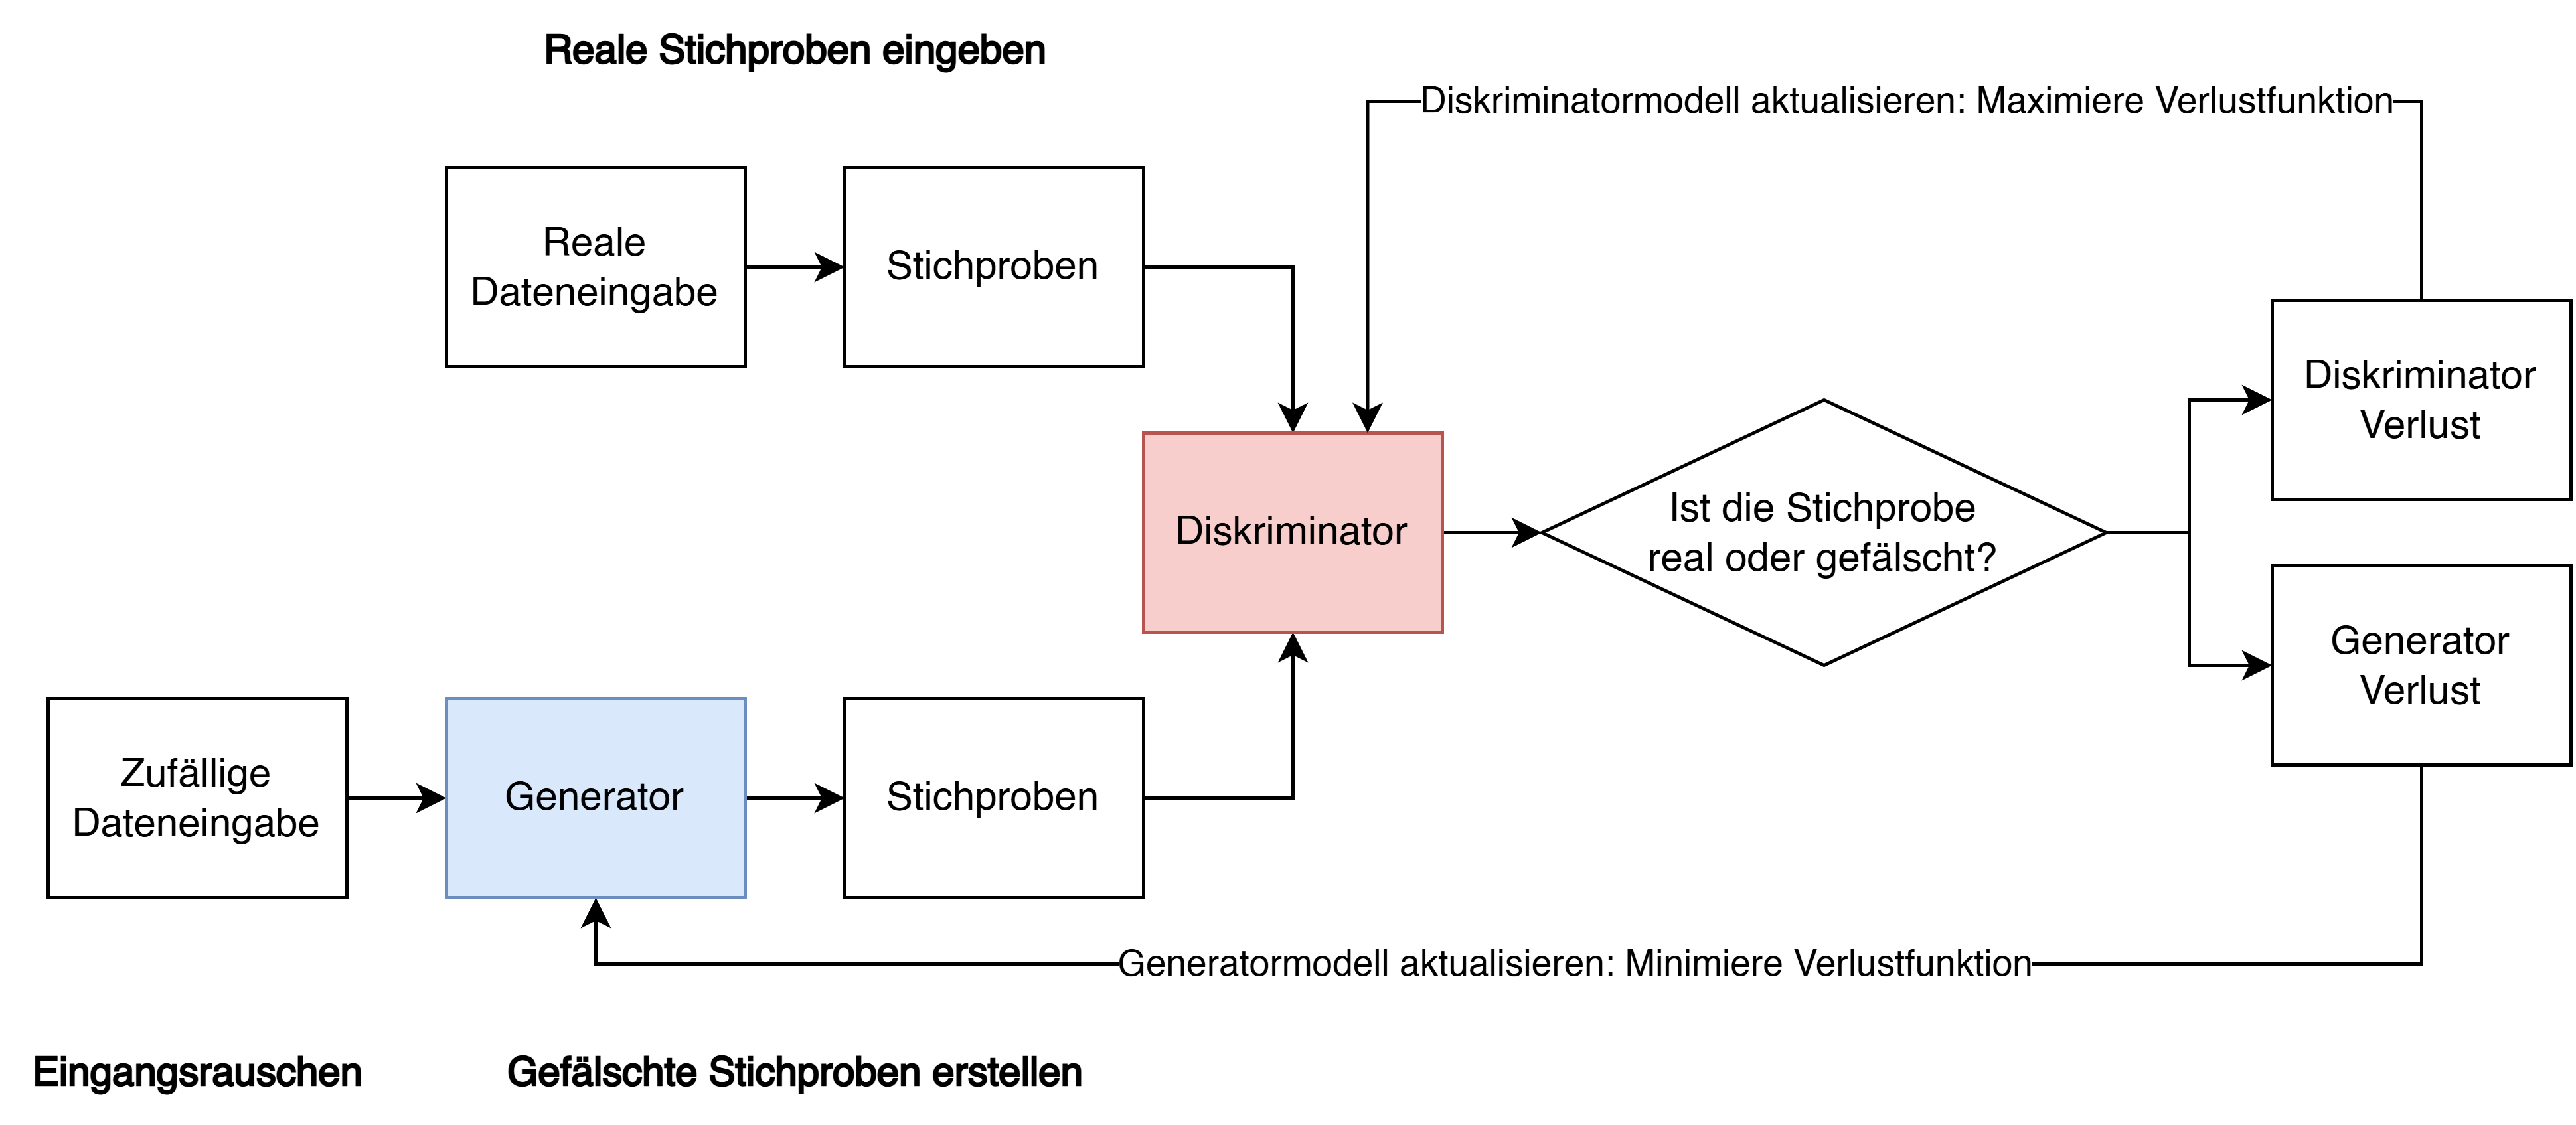
\includegraphics[width=\textwidth]{img/gan.png}
\caption[Architektur von Generative Adversarial Networks]{Architektur von Generative Adversarial Networks\footnotemark}
\label{fig:gan-architecture}
\end{center}
\end{figure}
\footnotetext{Eigene Darstellung in Anlehnung an \cite[672]{ramzan_generative_2024}}

Synthetische Daten finden in vielen Bereichen Anwendung. In der Forschung und Entwicklung bieten sie Daten für die Entwicklung und das Testen neuer Algorithmen und Modelle, ohne Datenschutzbestimmungen zu verletzen. In der Bildung und im Training können sie in Schulungen und Kursen verwendet werden, um realistische Datensätze zur Verfügung zu stellen, ohne sensible Informationen preiszugeben. In der Softwareentwicklung ermöglichen sie Entwicklern, Software mit repräsentativen Daten zu testen und zu validieren, ohne Zugriff auf echte Daten zu benötigen.

Die Nutzung synthetischer Daten bietet eine Reihe von Chancen. Einer der wichtigsten Vorteile stellt der hohe Datenschutz dar. Vollständig synthetische Daten enthalten keine echten personenbezogenen Informationen und sind daher frei von Datenschutzrisiken -- sofern sie qualitätsgeprüft sind und sorgfältig generiert wurden \cite[58]{hradec_multipurpose_2022}. Studien haben gezeigt, dass das Risiko einer Identitätsaufdeckung bei synthetischen Daten weit unter den üblichen Risikoschwellen liegt, selbst ohne darüber hinausgehende Sicherheits- und Datenschutzkontrollen \cite[9]{el_emam_evaluating_2020}. Zudem sind synthetische Daten in unbegrenzten Mengen verfügbar bzw. generierbar, was zweierlei Vorteile mit sich bringt: einerseits eine wichtige Grundlage für das Training datenhungriger KI-Modelle, andererseits erhebliche Aufwand- und Kosteneinsparungen im Vergleich zur Erhebung realer Daten. Darüber hinaus können synthetische Daten dazu dienen, Verzerrungen in Datensätzen zu reduzieren (z. B. hinsichtlich Alter, Geschlecht oder ethnischer Herkunft) und die Fairness darauf aufbauender Modelle zu erhöhen.

Trotz ihrer Vorteile gibt es auch Herausforderungen und Grenzen bei der Nutzung synthetischer Daten. Die Qualität synthetischer Daten hängt stark von den verwendeten Erzeugungstechniken und Modellen ab \cite[60]{hradec_multipurpose_2022}. Auch eine schlechte Qualität der Ursprungsdaten kann zu ungenauen oder irreführenden Ergebnissen führen \cite[2]{selvarajoo_towards_2024}. Die Akzeptanz und das Vertrauen in synthetische Daten sind ebenfalls nicht zu vernachlässigen \cite{van_hoorn_acceptance_2024}, insbesondere wenn deren Erzeugung und Eigenschaften nicht vollständig transparent sind. Nicht zuletzt können synthetische Daten in einigen Fällen nicht alle Besonderheiten und Nuancen der echten Daten vollständig erfassen, was ihre Nutzbarkeit einschränken kann \cite[5]{hao_synthetic_2024}.

\end{spacing}
\section{Vergleich mit traditionellen Anonymisierungsmethoden}
\label{sec:traditionelle-anonymisierung}
\begin{spacing}{1.5}

Eine der gängigsten Techniken zur Anonymisierung von Daten ist die Generalisierung. Dabei werden spezifische Werte durch weniger genaue, gröbere Werte ersetzt \cite[33]{schwartmann_praxisleitfaden_2022}. Beispielsweise könnte ein genaues Geburtsdatum durch das Geburtsjahr oder ein genauer Wohnort durch eine größere geografische Region ersetzt werden. Diese Methode hilft, die Identifizierbarkeit einzelner Personen zu verringern, indem detaillierte Informationen abstrahiert werden. Allerdings kann die Generalisierung die Präzision und Nutzbarkeit der Daten einschränken, da Nuancen und Details verloren gehen, die für bestimmte Analysen wichtig sein könnten.

Suppression ist eine weitere häufig verwendete Technik, bei der bestimmte Informationen vollständig entfernt oder durch Sonderzeichen (z. B. Asterisk) ersetzt werden, wenn sie als zu riskant für eine mögliche Re-Identifizierung angesehen werden \cite[1155]{lei_xu_information_2014}. Dies kann besonders effektiv sein, um sensible Daten zu schützen, wie beispielsweise individuelle Identifikationsnummern oder sensible medizinische Diagnosen. Der Nachteil dieser Methode liegt jedoch im erheblichen Informationsverlust, der auftreten kann, wenn große Mengen an Daten unterdrückt werden müssen, was die Nutzbarkeit der Datensätze stark beeinträchtigen kann.

Aggregation ist eine Technik, bei der Daten auf einer höheren Abstraktionsebene zusammengefasst werden \cite[11]{gumz_anonymisierung_2019}. Beispielsweise könnten individuelle Transaktionsdaten zu monatlichen oder jährlichen Summen aggregiert werden. Durch die Aggregation wird die Granularität der Daten reduziert, was das Risiko der Identifizierung einzelner Personen verringert. Diese Methode verbessert den Datenschutz, schränkt jedoch die Fähigkeit ein, detaillierte Analysen durchzuführen, da spezifische Informationen, die für tiefere Einsichten notwendig sein könnten, verloren gehen.

Ein weiteres herkömmliches Verfahren ist die Perturbation, bei der Daten durch Hinzufügen von Rauschen oder Zufallswerten modifiziert werden \cite[1155]{lei_xu_information_2014}. Diese Technik kann dazu beitragen, Muster zu verschleiern und somit die Re-Identifizierung zu erschweren, während die Gesamtstruktur der Daten erhalten bleibt. Allerdings muss darauf geachtet werden, dass das hinzugefügte Rauschen nicht so stark ist, dass es die Analysen und Interpretationen der Daten unbrauchbar macht.

Die Erzeugung synthetischer Daten beruht auf der Erstellung gänzlich neuer, künstlicher Datensätze und fällt damit in die Kategorie der Perturbationstechniken. Im Vergleich zu den anderen Methoden, die in der Regel mit einem größeren Informationsverlust einhergehen, ahmen synthetische Daten die statistischen Eigenschaften und Strukturen echter Daten nach, ohne tatsächliche personenbezogene Informationen zu enthalten. Diese Methode verwendet algorithmische Prozesse, um Daten zu generieren, die sich ähnlich wie die Originaldaten verhalten und aussehen, jedoch keine realen Personen repräsentieren.

\end{spacing}

\chapter{Analyse der Anforderungen und Problembeschreibung}
\label{cha:anforderungsanalyse}

\section{Problemdefinition}
\begin{spacing}{1.5}

Die Verarbeitung personenbezogener Daten in der öffentlichen Verwaltung stellt eine signifikante Herausforderung dar, insbesondere im Spannungsfeld zwischen Datenschutzanforderungen und dem Bedarf an analytisch nutzbaren Daten. Kommunale Datenbestände enthalten eine Vielzahl sensibler Informationen, die sowohl für die tägliche Verwaltungsarbeit als auch für strategische Analysen und Planungen unerlässlich sind. Die Hauptproblematik liegt darin, wie diese Daten sicher verarbeitet und gleichzeitig für verschiedene Analysezwecke genutzt werden können, ohne die Privatsphäre der Bürger zu gefährden.

Die herkömmlichen Methoden der Datenanonymisierung und Pseudonymisierung (vgl. Abschnitt \ref{sec:traditionelle-anonymisierung}) bieten zwar Ansätze, um den Schutz personenbezogener Daten zu gewährleisten, stoßen jedoch in der Praxis häufig auf Grenzen. Während Anonymisierungsverfahren darauf abzielen, personenbezogene Informationen unkenntlich zu machen, führen sie oft zu einem erheblichen Informationsverlust, der die Nützlichkeit der Daten für analytische Zwecke einschränkt. Pseudonymisierung kann zwar eine höhere Datenqualität bewahren, birgt aber weiterhin das Risiko der Re-Identifizierung, insbesondere wenn zusätzliche Informationen vorhanden sind, die zur Verknüpfung der Daten verwendet werden können. Diese Problematik wird durch die zunehmende Menge und Komplexität der gesammelten Daten noch verstärkt.

%Ein weiteres zentrales Problem ist die Akzeptanz und das Vertrauen in synthetische Daten innerhalb der öffentlichen Verwaltung. Entscheider und Analysten müssen überzeugt sein, dass synthetische Daten eine verlässliche und valide Grundlage für ihre Analysen bieten. Dies erfordert umfassende Tests und Validierungen, um die Qualität und Integrität der synthetischen Daten sicherzustellen.

\end{spacing}
\section{Zieldefinition und Erfolgskriterien}
\begin{spacing}{1.5}

Das Hauptziel dieser Arbeit besteht darin, die Rolle synthetischer Daten in kommunalen Datenbeständen zu untersuchen und zu evaluieren, wie diese Daten genutzt werden können, um den Datenschutz zu gewährleisten und gleichzeitig die analytische Nutzbarkeit zu verbessern. Dabei sollen die spezifischen Anforderungen und Herausforderungen, die sich aus der Anwendung synthetischer Daten in der öffentlichen Verwaltung ergeben, identifiziert und geeignete Lösungsansätze entwickelt werden. Es soll untersucht werden, wie synthetische Daten im Vergleich zu traditionellen Anonymisierungsmethoden abschneiden und ob sie eine verlässliche Alternative darstellen, um den Schutz personenbezogener Daten zu verbessern, ohne die Qualität und Nutzbarkeit der Daten zu beeinträchtigen.

Ein weiteres Ziel ist die praktische Implementierung und Bewertung synthetischer Daten am Beispiel der öffentlichen Verwaltung. Hierbei soll ein Synthesizer-Tool ausgewählt und spezifiziert werden, das in der Lage ist, qualitativ hochwertige synthetische Zensusdaten zu generieren. Diese Implementierung soll die theoretischen Überlegungen untermauern und konkrete Einblicke in die Anwendbarkeit und Leistungsfähigkeit synthetischer Daten in einem realen Szenario bieten.

Die Erfolgskriterien dieser Arbeit umfassen mehrere Dimensionen:

\begin{enumerate}
    \item Datenschutz: Die synthetischen Daten müssen die Datenschutzanforderungen gemäß \acrshort{dsgvo} und \acrshort{bdsg} erfüllen. Dies beinhaltet die Minimierung des Risikos einer Re-Identifizierung und den Schutz der Privatsphäre der betroffenen Personen.
    \item Datenqualität: Die synthetischen Daten sollen die statistischen Eigenschaften und Strukturen der Originaldaten möglichst genau widerspiegeln. Dies umfasst die Beibehaltung von Korrelationen, Verteilungen und anderen relevanten Datenmerkmalen, die für analytische Zwecke wichtig sind.\newpage
    \item Nutzbarkeit: Die synthetischen Daten müssen für die gleichen Analysen und Anwendungen geeignet sein wie die Originaldaten. Dies bedeutet, dass sie in der Praxis ähnliche Ergebnisse liefern und für die Entscheidungsfindung in der öffentlichen Verwaltung brauchbar sein müssen.
\end{enumerate}

Neben diesen Kriterien ist anzumerken, dass die organisatorische Implementierbarkeit sowie die Akzeptanz seitens der Beteiligten ebenfalls entscheidende Faktoren für den Erfolg synthetischer Daten in der öffentlichen Verwaltung darstellen. Diese Aspekte sind jedoch äußerst komplex und würden den Rahmen dieser Seminararbeit überschreiten. Daher werden sie in dieser Arbeit nicht näher untersucht und bleiben Gegenstand zukünftiger Forschungen.

\end{spacing}

\chapter{Implementierung am Beispiel der kommunalen Verwaltung}
\label{cha:implementierung}

\section{Konkretisierung der Problemstellung}
\begin{spacing}{1.5}

Die Nutzung von Zensusdaten in der öffentlichen Verwaltung stellt hohe Anforderungen an Datenschutz und Datensicherheit. Einerseits sind diese Daten äußerst wertvoll für analytische Zwecke, wie die Planung von Infrastrukturprojekten, die Bereitstellung von Sozialdiensten und die Verbesserung der öffentlichen Sicherheit. Andererseits müssen strenge Datenschutzrichtlinien eingehalten werden, um die Vertraulichkeit und Integrität der sensiblen Informationen zu gewährleisten.

Im Rahmen dieser Arbeit wird die Problematik der Nutzung realer Zensusdaten für Forschungszwecke beleuchtet. Traditionelle Methoden zur Anonymisierung stoßen häufig an ihre Grenzen, da sie nicht immer vollständig vor Re-Identifikationsrisiken schützen können. Dies führt zu einem Spannungsfeld zwischen der Notwendigkeit, detaillierte Daten zu verwenden, und der Pflicht, die Privatsphäre der Betroffenen zu schützen.

Die Lösung dieses Dilemmas könnte in der Verwendung synthetischer Daten liegen. Diese bieten die Möglichkeit, realistische, aber dennoch fiktive Daten zu generieren, die statistisch und strukturell den Originaldaten ähneln, jedoch keine direkten Rückschlüsse auf individuelle Personen zulassen. Die Frage, ob synthetische Zensusdaten eine praktikable Alternative zu realen Zensusdaten darstellen können, wird im weiteren Verlauf dieser Arbeit genauer untersucht.

\end{spacing}
\section{Auswahl und Spezifikation des Synthesizer-Tools}
\label{sec:synthesizer-tool-selection}
\begin{spacing}{1.5}

Für das Forschungsziel dieser Arbeit wurde die open-source Python-Library \textit{Synthetic Data Vault} (\acrshort{sdv}) ausgewählt \cite{synthetic_data_vault_2016}. \acrshort{sdv} bietet eine breite Palette an generativen Modellen wie Gaussian Copula, \acrshort{ctgan} und CopulaGAN, die qualitativ hochwertige synthetische Daten erzeugen können. Als Synthesizer wurde der \textit{CTGANSynthesizer} von \acrshort{sdv} verwendet. Dieses Modell nutzt \acrshort{gan}s, speziell das Conditional Tabular GAN-Modell (\acrshort{ctgan}), wie es von Xu et al. beschrieben wurde \cite{xu_modeling_2019}.

Es ist jedoch anzumerken, dass kommerzielle Lösungen wie Gretel oder Mostly AI aktuell noch überlegen sind \cite[60]{hradec_multipurpose_2022}, insbesondere hinsichtlich der Benutzerfreundlichkeit und der Tiefe automatisch generierter Reports und Analysen. Vor allem, wenn es darum geht, komplexere Tabellen mit einer Vielzahl von Einschränkungen, hoch kardinalen kategorialen Variablen und diskreten Daten zu verarbeiten, stoßen Open-Source-Lösungen an ihre Grenzen \cite[57]{hradec_multipurpose_2022}. Dennoch entwickelt sich das Feld der Open-Source-Lösungen schnell weiter, und es ist zu erwarten, dass in naher Zukunft wettbewerbsfähige Alternativen verfügbar sein werden.

Trotz der aktuellen Überlegenheit kommerzieller Lösungen genügt \acrshort{sdv} den Anforderungen dieser Studie. Es bietet die notwendige Datenqualität und Flexibilität, um die Synthesemethoden an die spezifischen Gegebenheiten der Zensusdaten anzupassen. Zudem stellt \acrshort{sdv} eine günstige Lösung dar, die ohne Lizenzkosten auskommt und somit besser in das Budget dieser Forschungsarbeit passt.

\end{spacing}
\section{Generierung synthetischer Zensusdaten}
\begin{spacing}{1.5}

Der zugrunde liegende Datensatz, der Census Income Dataset, wird von \acrshort{sdv} bereitgestellt und basiert auf dem ursprünglichen Census Income Dataset des UCI Machine Learning Repository \cite{misc_adult_2}. Die darin enthaltenen Daten wurden 1994 durch das United States Census Bureau erhoben und umfassen demografische und sozioökonomische Informationen von 32.561 Personen. In der Forschung wird dieser Datensatz häufig hergenommen, um Kausalitäten zu untersuchen, meist hinsichtlich der Frage, wovon das Einkommens einer Person abhängt\footnote{So etwa \cite{lazar_income_2004, islam_rana_investigation_2024, chakrabarty_statistical_2018}}. Die \acrshort{sdv}-Version dieses Datensatzes\footnote{Datensatz erreichbar unter: \url{https://sdv-demo-datasets.s3.amazonaws.com/SINGLE_TABLE/census_extended.zip}} erweitert jenen Ursprungsdatensatz um zusätzliche Spalten, einschließlich eines Quasi-Identifikators wie beispielsweise einer Adresse -- wobei diese fiktiv ist. Der Datensatz eignet sich als Beispiel für die Kommunalverwaltung aufgrund seiner umfassenden und vielfältigen Attribute, die typische Verwaltungsdaten widerspiegeln. So enthält er nicht nur demografische Informationen wie Alter, Geschlecht und Bildung, sondern auch sozioökonomische Merkmale wie Beruf, Arbeitszeit und Einkommensstufe.

\begin{table}[!htb]
    \centering\footnotesize
    \begin{tabular}{llllll}
        \toprule
        \\[-0.7em]
        age & workclass & education & race & income & address \\
        \\[-0.9em]
        \midrule
        \\[-0.7em]
        39 & State-gov & Bachelors & White & <=50K & 058 Wilson Inlet Apt. 470 Lake ...\\
        50 & Self-emp-not-inc & Bachelors & White & >50K & 9915 Andrew Road Ericashire ...\\
        38 & Private & HS-grad & White & <=50K & 4656 Tammy Terrace East Tonya ...\\
        53 & Private & 11th & Black & <=50K & 503 Danielle Dam South Melissa ...\\
        \\[-0.9em]
        \bottomrule
    \end{tabular}
    \caption[Auszug des verwendeten Datensatzes mit ausgewählten Spalten]{Auszug des verwendeten Datensatzes mit ausgewählten Spalten\footnotemark}
    \label{tab:census-data-sample}
\end{table}
\footnotetext{Eigene Darstellung}

\begin{figure}[ht]
\begin{center}
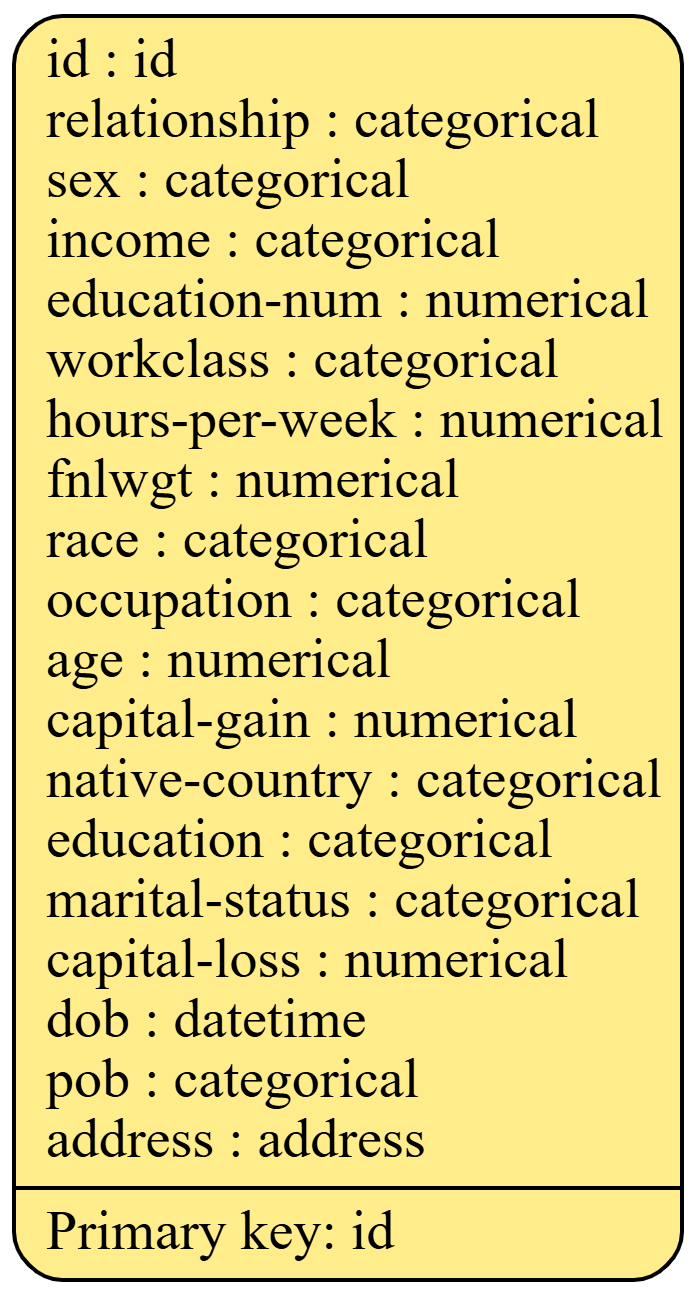
\includegraphics[width=0.24\textwidth]{img/metadata.png}
\caption[Beschreibung der Attribute inkl. Datentypen und Primärschlüssel]{Beschreibung der Attribute inkl. Datentypen und Primärschlüssel}
\label{fig:metadata}
\end{center}
\end{figure}

Nachdem die Metadaten (vgl. Abbildung \ref{fig:metadata}) festgelegt wurden, wird der im vorherigen Abschnitt \ref{sec:synthesizer-tool-selection} behandelte CTGANSynthesizer erstellt (vgl. Anhang 2). Mittels maschinellen Lernens wird der Synthesizer anschließend auf den gesamten 32.561 Einträgen trainiert. Unter Verwendung einer Tesla GPU 4\footnote{Bereitgestellt durch Google Colabs Compute Engine-Back-End} hat das Training 12 Minuten gedauert. Abschließend kann mithilfe der sample-Methode eine beliebige Anzahl an synthetischen Daten erzeugt werden, welche es im nächsten Kapitel zu evaluieren gilt.

\end{spacing}

\chapter{Evaluation}
\label{cha:evaluation}

\section{Bewertung der Datenqualität und -validität}
\begin{spacing}{1.5}

Insgesamt wurden 5.000 synthetische Daten generiert. \acrshort{sdv} verfügt über eingebaute Funktionen zur Bewertung der synthetischen Daten und zur Gewinnung weiterer Erkenntnisse. Die \acrshort{sdv}-Diagnose führt einige grundlegende Validitätsprüfungen\footnote{\url{https://docs.sdv.dev/sdv/single-table-data/evaluation/diagnostic\#whats-included}} durch:

\begin{itemize}
  \item Alle Primärschlüssel müssen eindeutig sein.
  \item Stetige Werte müssen mit den Minimal- und Maximalwerten der realen Daten übereinstimmen.
  \item Diskrete Spalten müssen die gleichen Kategorien haben wie die echten Daten.
\end{itemize}

Die \acrshort{sdv}-Diagnose ergab, dass die generierten Daten zu 100 \% valide sind. Eine daraufhin ausgeführte Auswertung der Datenqualität (evaluate\_quality) ergab, dass die synthetischen Daten zu 86,1 \% mit den realen Daten hinsichtlich ihrer statistischen Eigenschaften (z. B. Korrelation \& Randverteilung) übereinstimmen. Eine detaillierte Aufschlüsselung der Korrelationswerte kann Tabelle \ref{tab:correlation-detailled} entnommen werden.

\newpage

\begin{table}[!htb]
    \centering\footnotesize
    \begin{tabular}{lll}
        \toprule
        \\[-0.7em]
        Attribut & Datentyp & Korrelation [\%] \\
        \\[-0.9em]
        \midrule
        \\[-0.7em]
        income & kategorisch & 0.982810 \\
        age & nummerisch & 0.956845 \\
        sex & kategorisch & 0.945395 \\
        dob & datetime & 0.947869 \\
        education-num & nummerisch & 0.952392 \\
        workclass & kategorisch & 0.933288 \\
        hours-per-week & nummerisch & 0.927463 \\
        education & kategorisch & 0.924603 \\
        marital-status & kategorisch & 0.904812 \\
        race & kategorisch & 0.901783 \\
        relationship & kategorisch & 0.872116 \\
        fnlwgt & nummerisch & 0.865818 \\
        pob & kategorisch & 0.808084 \\
        capital-loss & nummerisch & 0.800251 \\
        native-country & kategorisch & 0.799960 \\
        occupation & kategorisch & 0.770835 \\
        capital-gain & nummerisch & 0.689690 \\
        \\[-0.9em]
        \bottomrule
    \end{tabular}
    \caption[Detaillierte Korrelationswerte der synthetischen Daten]{Detaillierte Korrelationswerte der synthetischen Daten\footnotemark}
    \label{tab:correlation-detailled}
\end{table}
\footnotetext{Eigene Darstellung}

\end{spacing}
\section{Vergleichende Analyse mit realen Daten}
\label{sec:comparing-analysis}
\begin{spacing}{1.5}

Vergleicht man die generierten synthetischen Daten mit den realen Daten, so fällt zunächst auf, dass diese auf den ersten Blick nicht voneinander unterscheidbar sind -- abgesehen von der Reihenfolge der Spalten (vgl. Anhang 1). Im ursprünglichen Datensatz war mit der Adresse auch ein sensitives (wenn auch fiktives) Attribut enthalten. Dieses wurde durch den Synthesizer automatisch erkannt und vollkommen anonymisiert, indem mithilfe der Python-Bibliothek \textit{Faker} grundlegend neue, gefälschte Werte erstellt werden, die lediglich der Syntax des Originals entsprechen.

Eine detaillierte Betrachtung der Datenqualität erfolgt anhand mehrerer Vergleichsdiagramme. Abbildung \ref{fig:real-vs-synthetic-age} zeigt die Altersverteilungen in den realen und synthetischen Datensätzen. Man erkennt, dass die allgemeine Form der Verteilung in beiden Datensätzen sehr ähnlich ist, was darauf hinweist, dass der Synthesizer die Altersstruktur der Bevölkerung gut reproduziert hat.  Auffällig ist, dass die synthetischen Daten eine höhere relative Häufigkeit in der Altersgruppe von etwa 35 Jahren aufweisen und zwei weitere Hochpunkte bei etwa 22 und 46 Jahren zeigen. Im Vergleich dazu sind die realen Daten gleichmäßiger verteilt. Diese Auffälligkeit kann auf den Synthesizer selbst zurückgeführt werden, welcher dazu neigt, bestimmte Muster zu glätten, zu extrapolieren oder mit Rauschen zu überlagern\footnote{\url{https://docs.sdv.dev/sdv/multi-table-data/evaluation/data-quality\#interpreting-the-score}}.

\begin{figure}[ht]
\begin{center}
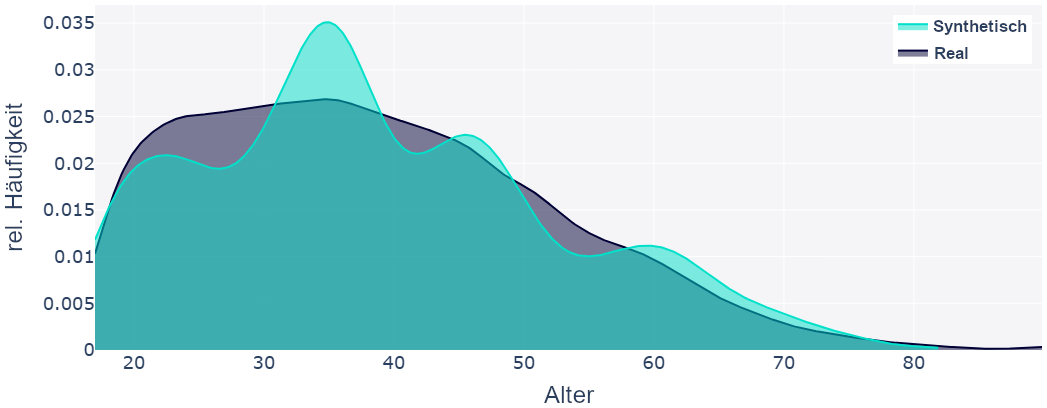
\includegraphics[width=\textwidth]{img/real-vs-synthetic-age.png}
\caption[Verteilung des Attributs \textit{age} in realen und synthetischen Daten]{Verteilung des Attributs \textit{age} in realen und synthetischen Daten}
\label{fig:real-vs-synthetic-age}
\end{center}
\end{figure}

\begin{figure}[ht]
\begin{center}
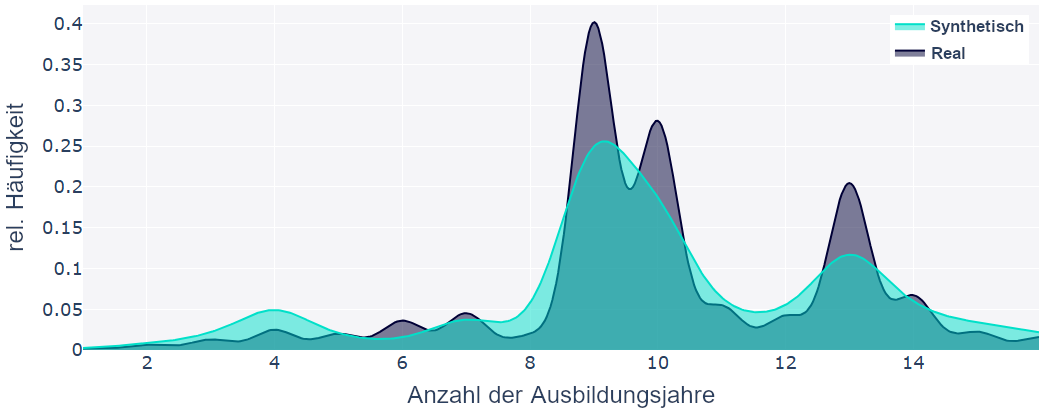
\includegraphics[width=\textwidth]{img/real-vs-synthetic-education.png}
\caption[Verteilung des Attributs \textit{education-num} in realen und synthetischen Daten]{Verteilung des Attributs \textit{education-num} in realen und synthetischen Daten}
\label{fig:real-vs-synthetic-education}
\end{center}
\end{figure}

Ein ähnliches Phänomen ist in Abbildung \ref{fig:real-vs-synthetic-education} zu beobachten. Im Gegensatz zur Verteilung des Alters zeigt die Verteilung des Attributs \textit{education-num} in den synthetischen Daten jedoch eine deutlich glattere Kurve. Dies deutet darauf hin, dass der Synthesizer hier eine stärkere Glättung vorgenommen hat, um die Verteilung der Bildungsniveaus nachzubilden. Während die reale Datenverteilung kleine Schwankungen und Unregelmäßigkeiten aufweist, sind diese in den synthetischen Daten weitgehend geglättet worden. Dies kann dazu führen, dass bestimmte Feinheiten der realen Daten nicht vollständig in den synthetischen Daten widergespiegelt werden, was bei der Interpretation und Verwendung der synthetischen Daten berücksichtigt werden muss.

\begin{figure}[ht]
\begin{center}
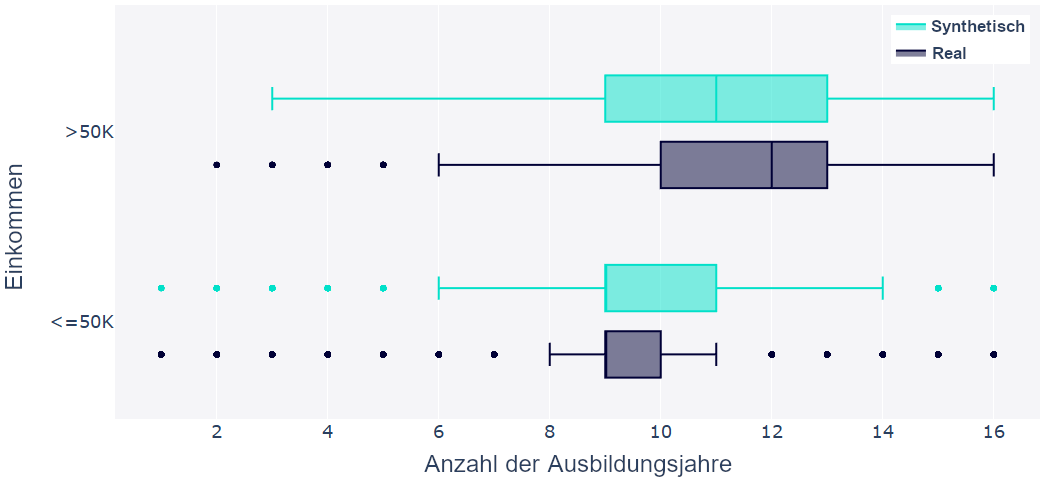
\includegraphics[width=\textwidth]{img/income-vs-education.png}
\caption[Attribut \textit{income} in Abhängigkeit zum Attribut \textit{education-num}]{Attribut \textit{income} in Abhängigkeit zum Attribut \textit{education-num}}
\label{fig:income-vs-education}
\end{center}
\end{figure}

Abbildung \ref{fig:income-vs-education} zeigt mehrere Box-Plots und visualisiert die Korrelation zwischen Bildung und Einkommen sowohl in den realen als auch in den synthetischen Daten. Die synthetischen Daten reproduzieren die positive Korrelation zwischen höheren Bildungsabschlüssen und höherem Einkommen, die auch in den realen Daten zu beobachten ist. Anhand der Box-Plots fällt jedoch auf, dass die Streuung in den synthetischen Daten größer ist.

\end{spacing}

\chapter{Diskussion der Ergebnisse}
\label{cha:diskussion}

\section{Herausforderungen und Chancen für die öffentliche Verwaltung}
\begin{spacing}{1.5}

Die Nutzung synthetischer Daten in der öffentlichen Verwaltung bietet sowohl Herausforderungen als auch Chancen. Eine der größten Herausforderungen ist die Sicherstellung der Datenqualität und -validität. Die Analyse hat gezeigt, dass die synthetischen Daten zu 100 \% valide sind und eine Übereinstimmung von etwa 86 \% mit den realen Daten hinsichtlich ihrer statistischen Eigenschaften aufweisen. Diese Werte sind vielversprechend, aber es bleibt eine Restabweichung, die bei kritischen Entscheidungen berücksichtigt werden muss.

Eine weitere Herausforderung ist die Akzeptanz der synthetischen Daten innerhalb der Verwaltung. Um diese Daten als valide Grundlage für Analysen zu akzeptieren, ist Transparenz in der Datenentstehung und Vertrauen in die Qualität und Sicherheit der Daten erforderlich. Dieses Vertrauen könnte durch Schulungen und ausgewählte Pilotprojekte gefördert werden, die den Mitarbeitern der Verwaltung die Prinzipien und Methoden der Datensynthese näherbringen. Zudem ist es wichtig, regelmäßige Audits und Qualitätskontrollen durchzuführen, um die Zuverlässigkeit der synthetischen Daten zu gewährleisten.

Auf der anderen Seite bieten synthetische Daten erhebliche Chancen. Sie ermöglichen es, detaillierte Analysen durchzuführen, ohne gegen Datenschutzrichtlinien zu verstoßen. Insbesondere in Bereichen wie dem Bürger- oder Gesundheitswesen können synthetische Daten dazu beitragen, sensible Informationen zu schützen und gleichzeitig wertvolle Erkenntnisse zu gewinnen, die zur Verbesserung der öffentlichen Dienstleistungen beitragen.

\end{spacing}
\section{Grenzen und Limitationen der Arbeit}
\begin{spacing}{1.5}

Obwohl diese Arbeit wertvolle Einblicke in die Nutzung synthetischer Daten in der kommunalen Verwaltung bietet, gibt es einige Grenzen und Limitationen, die beachtet werden müssen.

Erstens stützt sich die Arbeit lediglich auf den Census Income Datensatz. Während dieser Datensatz als repräsentativ für viele demografische und sozioökonomische Merkmale gilt, kann er nicht alle möglichen Variablen und Kontexte abdecken, die in unterschiedlichen kommunalen Anwendungen relevant sein könnten. Die Ergebnisse dieser Arbeit sind somit möglicherweise nicht ohne weiteres auf andere Datensätze oder Szenarien übertragbar.

Zweitens basieren die Implementierung und Analyse auf spezifischen technischen Rahmenbedingungen und den Eigenschaften des gewählten \acrshort{ctgan}-Synthesizer-Tools von \acrshort{sdv}. Andere Tools oder technische Implementierungen könnten zu unterschiedlichen Ergebnissen führen. Die Ergebnisse und Schlussfolgerungen dieser Arbeit sind daher primär auf das verwendete Tool und die damit verbundenen Konfigurationen beschränkt.

Ein weiterer Punkt ist der eingeschränkte Fokus der Arbeit. Sie konzentriert sich hauptsächlich auf die technische Machbarkeit und die Qualität der generierten synthetischen Daten. Aspekte wie die organisatorische Implementierung, die Schulung von Mitarbeitern oder die rechtlichen Rahmenbedingungen werden nur am Rande behandelt und bleiben weitgehend unberücksichtigt. Diese Faktoren sind jedoch entscheidend für die praktische Umsetzung und Akzeptanz synthetischer Daten in der öffentlichen Verwaltung.

Nicht zuletzt wurden die ethischen und sozialen Implikationen der Nutzung synthetischer Daten in dieser Arbeit nicht eingehend untersucht. Aspekte wie die Wahrnehmung und Akzeptanz durch die Öffentlichkeit, mögliche Verzerrungen oder Diskriminierungen durch synthetische Daten und deren Auswirkungen auf die gesellschaftliche Gleichheit bleiben offen und bedürfen weiterer Forschung.

\end{spacing}

\chapter{Fazit und Ausblick}
\label{cha:fazit}
\begin{spacing}{1.5}

Die vorliegende Seminararbeit befasste sich mit der Nutzung synthetischer Daten in der öffentlichen Verwaltung, einem Thema von wachsender Bedeutung angesichts der zunehmenden Digitalisierung und des steigenden Bedarfs an datengestützten Entscheidungsprozessen.

Zusammenfassend lässt sich feststellen, dass synthetische Daten erhebliche Vorteile bieten, insbesondere in Bezug auf den Datenschutz und die Möglichkeit, detaillierte Analysen durchzuführen, ohne die Privatsphäre der Bürger zu gefährden. Die Analyse der synthetischen Daten zeigte eine hohe Validität und eine beachtliche Übereinstimmung mit realen Daten, was ihre Nützlichkeit unterstreicht. Jedoch wurden auch Grenzen und Limitationen identifiziert, die die Genauigkeit und Generalisierbarkeit der Ergebnisse beeinflussen können.

Ein zentraler Punkt der Arbeit war die Identifizierung der Herausforderungen, die mit der Nutzung synthetischer Daten verbunden sind. Dazu gehören die Sicherstellung der Datenqualität, die Akzeptanz der Daten innerhalb der Verwaltung und die technischen sowie organisatorischen Anforderungen an die Implementierung. Diese Herausforderungen erfordern eine sorgfältige Planung und die Entwicklung geeigneter Strategien, um die breite Anwendung synthetischer Daten erfolgreich zu gestalten.

Ein Blick in die Zukunft zeigt, dass synthetische Daten eine zunehmend wichtige Rolle in der öffentlichen Verwaltung spielen könnten. Zukünftige Forschung sollte sich darauf konzentrieren, die Methoden der Datensynthese weiter zu verbessern und die Anwendungsszenarien in der Praxis zu erweitern. Insbesondere detaillierte Fallstudien könnten wertvolle Einblicke in die praktischen Herausforderungen und Erfolge bei der Nutzung synthetischer Daten liefern.

\end{spacing}

\pagestyle{plain}

\newpage
\chapter*{Anhang}
\label{cha:anhang}
\addcontentsline{toc}{chapter}{Anhang}

\section*{Anhang 1}
\label{sec:anhang-1}

\begin{figure}[ht]
\begin{center}
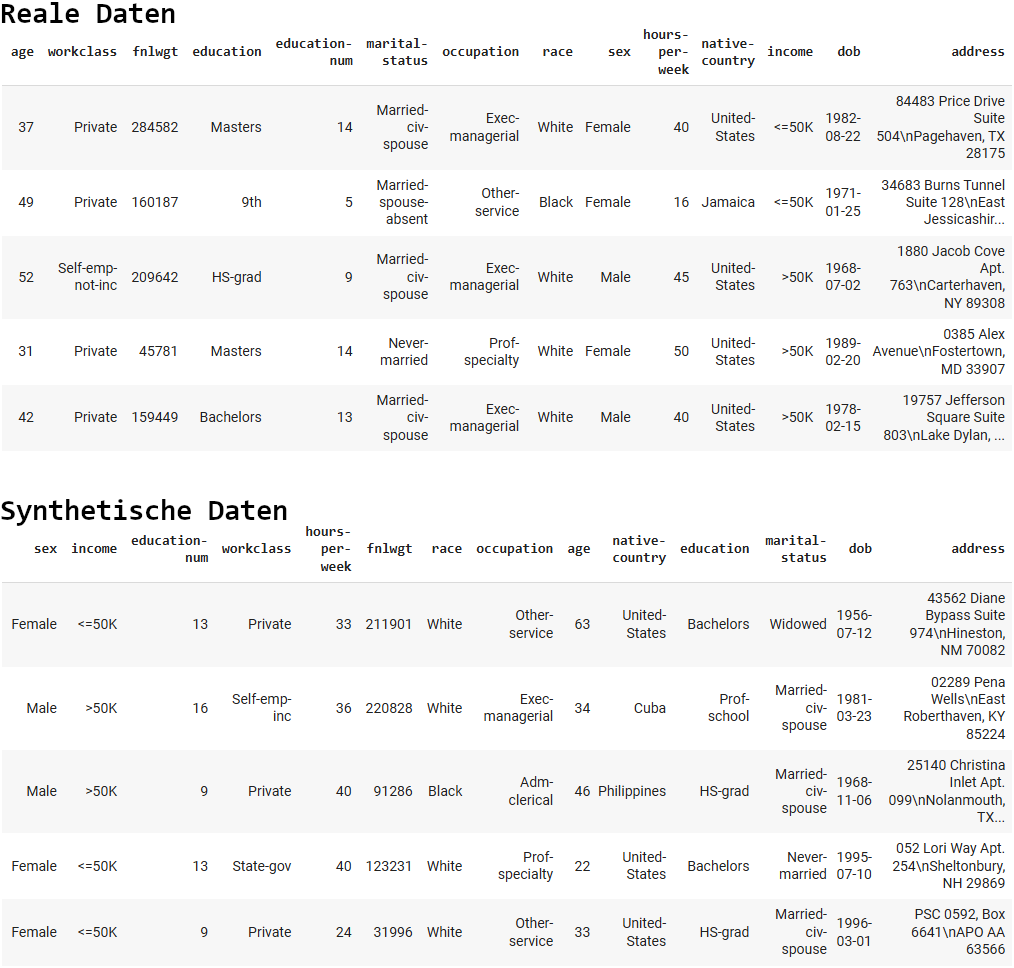
\includegraphics[width=\textwidth]{img/real-vs-synthetic-data.png}
\caption[Gegenüberstellung realer und synthetischer Daten]{Gegenüberstellung realer und synthetischer Daten\footnotemark}
\label{fig:real-vs-synthetic}
\end{center}
\end{figure}
\footnotetext{Eigene Darstellung}

\newpage
\section*{Anhang 2}
\label{sec:anhang-2}

\inputminted{python}{lst/sdv.py}
\captionof{listing}{Python-Implementierung zur Erstellung synthetischer Zensusdaten}

\pagestyle{fancy}

%Literaturverzeichnis
\setcounter{biburllcpenalty}{7000}
\setcounter{biburlucpenalty}{8000}
%\addcontentsline*{toc}{section}{Literatur}
%\section*{Literatur}
\printbibliography[heading=bibintoc, title={Literatur}]
%\printbibliography

\newpage
\chapter*{Eigenständigkeitserklärung}
\addcontentsline{toc}{chapter}{Eigenständigkeitserklärung}
\begin{spacing}{1.5}
Hiermit versichere ich, dass ich die angemeldete Prüfungsleistung in allen Teilen eigenständig ohne Hilfe von Dritten anfertigen und keine anderen als die in der Prüfungsleistung angegebenen Quellen und zugelassenen Hilfsmittel verwenden werde. Sämtliche wörtlichen und sinngemäßen Übernahmen inklusive KI-generierter Inhalte werde ich kenntlich machen.\par
Diese Prüfungsleistung hat zum Zeitpunkt der Abgabe weder in gleicher noch in ähnlicher Form, auch nicht auszugsweise, bereits einer Prüfungsbehörde zur Prüfung vorgelegen; hiervon ausgenommen sind Prüfungsleistungen, für die in der Modulbeschreibung ausdrücklich andere Regelungen festgelegt sind.\par
Mir ist bekannt, dass die Zuwiderhandlung gegen den Inhalt dieser Erklärung einen Täuschungsversuch darstellt, der das Nichtbestehen der Prüfung zur Folge hat und daneben strafrechtlich gem. § 156 StGB verfolgt werden kann. Darüber hinaus ist mir bekannt, dass ich bei schwerwiegender Täuschung exmatrikuliert und mit einer Geldbuße bis zu 50.000 EUR nach der für mich gültigen Rahmenprüfungsordnung belegt werden kann.\par
Ich erkläre mich damit einverstanden, dass diese Prüfungsleistung zwecks Plagiatsprüfung auf die Server externer Anbieter hochgeladen werden darf. Die Plagiatsprüfung stellt keine Zurverfügungstellung für die Öffentlichkeit dar.\\[2cm]
\parbox{4cm}{\hrule \strut \centering\footnotesize Ort, Datum} \hfill
\parbox{4cm}{\hrule \strut \centering\footnotesize Unterschrift}
\end{spacing}

\end{document}